%% $RCSfile: proj_report_outline.tex,v $
%% $Revision: 1.2 $
%% $Date: 2010/04/23 02:40:16 $
%% $Author: kevin $

\documentclass[11pt
              , a4paper
              , twoside
              , openright
              ]{report}


\usepackage{float} % lets you have non-floating floats

\usepackage{url} % for typesetting urls

%
%  We don't want figures to float so we define
%
\newfloat{fig}{thp}{lof}[chapter]
\floatname{fig}{Figure}

%% These are standard LaTeX definitions for the document
%%                            
\title{Interactive 3D Visualisation of Exoplanets}
\author{Owen Bannister, 300172912}

%% This file can be used for creating a wide range of reports
%%  across various Schools
%%
%% Set up some things, mostly for the front page, for your specific document
%
% Current options are:
% [ecs|msor]              Which school you are in.
%
% [bschonscomp|mcompsci]  Which degree you are doing
%                          You can also specify any other degree by name
%                          (see below)
% [font|image]            Use a font or an image for the VUW logo
%                          The font option will only work on ECS systems
%
\usepackage[font,ecs,mcompsci]{vuwproject}
\usepackage{graphicx}
\usepackage{pdfpages}
% You should specifiy your supervisor here with
     \supervisor{Stuart Marshall}
% use \supervisors if there is more than one supervisor

% Unless you've used the bschonscomp or mcompsci
%  options above use
   \otherdegree{Bachelor of Software Engineering with Honors}
% here to specify degree

% Comment this out if you want the date printed.
\date{}

\begin{document}

% Make the page numbering roman, until after the contents, etc.
\frontmatter

%%%%%%%%%%%%%%%%%%%%%%%%%%%%%%%%%%%%%%%%%%%%%%%%%%%%%%%

%%%%%%%%%%%%%%%%%%%%%%%%%%%%%%%%%%%%%%%%%%%%%%%%%%%%%%%

\begin{abstract}


We have large amounts of information about planets outside of our solar system. This can be accessed from a database by anyone. However this information is complex and cannot be easily understood by laypeople. This is a problem as it means that the information gained about these planets is not being used effectively to convey the intended information to the masses. To resolve this a visualisation has been created that can convey this information in a way that interested lay people can understand. This visualisation can be used as an information source for those wanting to increase their knowledge about the planets residing outside of our solar system. This report outlines the project carried out, the planning and decisions made, the visualisation created, and its evaluation to discover its effectiveness at fullfilling the goals driving its creation.


\end{abstract}

%%%%%%%%%%%%%%%%%%%%%%%%%%%%%%%%%%%%%%%%%%%%%%%%%%%%%%%

\maketitle

\include{acknowledge}

\tableofcontents

% we want a list of the figures we defined
\listof{fig}{Figures}

%%%%%%%%%%%%%%%%%%%%%%%%%%%%%%%%%%%%%%%%%%%%%%%%%%%%%%%

\mainmatter

%%%%%%%%%%%%%%%%%%%%%%%%%%%%%%%%%%%%%%%%%%%%%%%%%%%%%%%

% individual chapters included here
\chapter{Introduction}\label{C:intro}
This project seeks to design, implement, and evaluate an interactive 3D visualisation software system for displaying the content in the Kepler Exoplanets dataset. The deliverable is intended as a standalone 3D visualisation system with two modes of interaction, keyboard and mouse or Microsoft Xbox Kinect sensor ((REF)). The resulting visualisation will convey the information in the dataset in a way that the target users, laypeople who have an interest in astronomy, can understand and interact with.
\section{Motivation}
There are many planets that have been located outside of our own solar system, these are
called exoplanets, these are referred to interchangeably as planets and exoplanets for the remainder of this report
. This project seeks to develop and evaluate an interactive 3D visualisation
software system for the Kepler exoplanets dataset [28]. This visualisation will convey information
in a way that the target users, laypeople who have an interest in astronomy, can
understand.
\section{Problem statement}
The complex nature of the data involved in this project causes a range of problems revolving around understandability to arise, which this project attempts to address. The following subsections outline these in detail.
\subsection{Understanding the content in the dataset}
Understanding and analysing large datasets whose size defies simplistic or trivial analysis is a known issue that many areas of research are attempting to address, these areas of research range from data mining to visualisations in order to discover or highlight important features in the data so that people can more efficiently use it. 
\\\\
Humans often rely on visualisation when we solve problems. We create an image in our mind of a situation in order to make sense of it http://nrich.maths.org/6447.~ This allows for a much more comprehensive understanding of the content being visualised. The content in the dataset used for this project is made up of records of every exoplanet discovered by the Kepler Mission. Each of which contains 46 fields. It is next to impossible for someone to internally visualise so much information, most of which is floating point numbers.This means that an external way of visualising it is needed, which is the problem that this project attempts to address. 
\clearpage
\begin{figure}[h!]
  \centering
      
\includegraphics[width=0.8\textwidth]{images/data.png}
  \caption{Dataset to be visualised}
\end{figure}

\subsection{Comprehension of planetary information}
Much of the information regarding planets is cryptic and unintuitive, this make its understandability difficult. Visualisations in general attempt to address this issue by displaying information in a way that conveys the information in simplistic ways which allows improved user comprehension.

\subsection{Existing solutions lack functionality}
Existing data visualisation techniques using this exoplanet dataset lack the ability to display sufficient detail on each exoplanet and do not provide answers to questions that can be answered by the Exoplanet attributes in the dataset. Existing solutions display only the size, temperature, and orbital information about the exoplanets. While this is useful information that informs users of important facts about the planets, it does leave a lot of potential information unseen and overlooked, for example, information about the type of planet, planets with similar traits, solar system information, similarity to earth and habitability. This project will therefore be focused on researching, implementing, and evaluating a new interactive visualisation system that will display additional information to users not included in previous visualisation systems.

\subsection{Effective user interaction with visualisation}
A visualisation that solely displays information without effective methods of interaction limits the immersive qualities that keeps users engaged. To address this interactive visualisations emerged, generally these visualisations allow users to modify the representation of information rather than the information itself. This means allowing user control some property of how the data is represented, be it something simple as the layout of elements or something more complex. Many mediums of interaction are possible from the mundane keyboards, mice, or touchpads to the more esoteric wired gloves, motion sensors, and omnidirectional treadmills or even a combination of a range of devices.
\\\\
With interactive visualisations, response time of the system to user actions is important and so changes made by the user must be incorporated into the visualization in a timely manner. Experiments have shown that a delay of more than 20 ms between when input is provided and a visualisation is updated is noticeable by most people ((REFERENCE)~). Thus it is important for an interactive visualization to provide a rendering based on human input within this time frame or else risk breaking user immersion.
\\\\

When the information being presented is altered, the visualization is usually part of a feedback loop. For example, consider an aircraft avionics system where the pilot inputs roll, pitch, and yaw and the visualization system provides a rendering of the aircraft's new attitude. Another example would be a scientist who changes a simulation while it is running in response to a visualization (see Visualization) of its current progress. This is called computational steering.

\section{Key issues project addresses}
To summarize the above sections, this project addresses the following key issues:
\begin{enumerate}
 \item[I1.] Content in database form is difficult to view and understand.
 \item[I2.] Planetary information is complex and difficult to comprehend without a visual reference.
 \item[I3.] Existing visualisations for this dataset have minimal functionality and have lacking usability.
 \item[I4.] User interaction is needed in a visualisation to make the most of data displayed.
\end{enumerate}

\section{Contributions of this project}
This project will provide an extension of the Kepler Visualisation Tool \cite{kepler_github} that conveys more information and is easier for users to interact with than the original. This extension will be evaluated by a user experiment to ensure that it is successful in conveying the information contained in the dataset.
\\\\
The work and research completed for this project will allow for further improvement by other developers and researchers to extend and improve the visualisation created. This will provide further exposure of the Kepler dataset which will encourage learning about Exoplanets.


\chapter{Project Methodologies}\label{C:m}

\section{Project management approach}
Following a structured project management approach is important as it avoids the problem caused by following a code-and-fix approach as described  as 1) write some code. 2) Fix the problems in the code \cite{boehm}. By following a process model it encourages thinking about requirements, design, and testing before coding is commenced. 
\\\\
The project methodology chosen for this project was a customized Spiral Model made up of requirements analysis, design, implementation, and evaluation phases as shown in the below figure. The reason for limiting the model to these 4 phases was because....  
\begin{figure}[h!]
  \centering
      \includegraphics[width=0.6\textwidth]{images/spiral_model.png}
  \caption{Spiral process model followed}
\end{figure}
Using a spiral model allowed me to produce a deliverable feature at the end of each iteration of the model, this ensured that I did not become delayed or stuck in my development. By using this methodology it also allowed me to prioritize the features that were the most important to the visualisation which reduced the risk that there would be missing or incomplete components at the end of the project. 
\\\\
The advantages of this methodology over other choices such as the waterfall model or an agile approach such as Scrum was that it provided me with the benefits of a structured work flow that is a feature of the waterfall model as well as a flexible iterative process that is a feature of Agile methodologies. Following a pure waterfall methodology would not have allowed me to iteratively design, develop, and evaluate each feature which would have forced more upfront design which limits flexibility and support for changing requirements and design as was needed for this project. Following a pure agile approach would not have been optimal as most Agile methodologies are more beneficial to projects that have a team working on them. As it was I was agile in my approach to the project as I produced a deliverable at the end of each of the cycles of the spiral model and responded to change in the form of feedback and ideas from the supervisor of the project.
\\\\
This project management technique supported the creation of a visualisation as it allowed the flexibility to add and remove components into the visualisation as they were discovered to be beneficial or not. It also supported the expansion of the project brief to include using a kinect sensor in order to control the visualisation. The choice of this project management approach meant that whilst I had the freedom to explore visualisation options I also had a structured software development life cycle to guide me and provide the project through the necessary steps to end in completion of each component.
\\\\
By supporting this project methodology with other project management tools such as Gantt charts [APPENDIX] and work breakdown structures(WBS) [APPENDIX], it encouraged efficient documentation of planning and work completed in the project as well as displaying the upcoming stages required to complete the project.
\\\\
Weekly meetings with the supervisor of the project, Dr Stuart Marshall, were used to provide guidance and ideas for innovation of the visualisation throughout the project. These meeting ensured that vital components and deliverables were implemented in the required timeframe and also provided a sounding board for ideas for elements to be included in the visualization. Another important aspect of having an involved supervisor was that he provided me the guidance of an experienced academic which was indispensable when navigating the administrative side of organizing delicate matters such as ethics approval for human evaluation of the visualisation.


\section{Key difficulties in project}
As this project builds upon a previous system much of the existing code and execution flow needs to be modified. This requires understanding of how the system was originally built and designed. Because this system does not have any unit or integration tests, going ahead without a comprehensive knowledge of the core functionality would be foolish.
\\\\
Encountered errors in Processing framework due to number of elements needing to be displayed on screen. 
\\\\
Having a time constraint of 300 hours for this project over the course of a year meant that prioritization of visualization features needed to be made to ensure that 
\\\\
Libraries used for gesture detection in kinect are opensource in order to work with processing did not have decent detection
\chapter{Requirements Analysis}\label{Chap:ra}
To guide the creation of the visualisation a user oriented design approach was
used \cite{AboutFace3}, in particular making use of user models (personas). These personas were
created to give a sense of empathy and understanding for the foreseen users of
the visualisation in order to better understand the requirements and design
decisions to be made. 

The visual design of the visualisation was based heavily on User Centered Design as it
provided a method of user interface design as well as visualisation design. User
Centered Design is a process in which the needs, wants, and limitations of the
end users of a system are given extensive attention. To achieve this, personas
were created (also known as archetypal users), which are a personification the
needs of a larger group of related users. These personas act as stand-ins for
real users, describing them in terms of their goals and personal
characteristics, and although they are fictitious, they are based on knowledge
of real users. This design methodology supported my understanding of how users
were likely to use the visualisation.

An additional tool used during requirements analysis was User Scenarios which
describe the foreseeable interactions of the user personas with the
visualisation. A scenario is made up of a functional goal for the visualisation
and describes how it is carried out by a persona. Both of these tools force you
to think about the tasks needed for the visualisation and their context in the
system as a whole. Once the personas and scenarios have been completed you can
then start to design specific elements of the user interface and visualisation
based on the requirements and interactions described in the scenarios. The User
Models and User Scenarios for this project are described in the following
sections.


\section{User models}
Below are the two personas that were used in the design of the visualisation for
this project. They depict users that would use the visualisation in the context
of a terminal or display in an observatory environment. These personas  can be
validated during evaluation of the visualization by finding real users that
match the core values of the personas.Although this visualisation would be
suited towards teaching childeren about stelar information they were not
focussed on during its planning. This was because due to the increased ethical
complexity with carrying out an evaluation with childeren. This could be done in
the future once the visualisation is deemed successfull. 

\subsection{John Truman (Primary Persona - The interested layperson)}\
24 year old John is interested in planets and space and has a basic knowledge
about both. He frequently visits attractions catering to this interest at
locations such as planetariums and observatories. Some of his favourite things
to do when visiting these attractions is to go to the computer terminals that
allow users to choose what information they see.

John is used to playing computer games and using visualisations and is not
overwhelmed understanding and using new systems. He finds that he learns better
when provided with visual examples than when reading or listening to
information. John is most comfortable using keyboard and mouse when interacting
with a computer.

\subsubsection{Scenario 1: View planets ordered by their similarity to Earth}
 When John first sees the system the first thing he notices is that there are
many planets orbiting what looks like a star. He doesn't have any point of
reference for these planets so their sizes, colours, and movement speeds are
meaningless. By providing a way of comparing the planets to Earth it gives a
point of reference which is well documented and known by most.
 
 {\bf Procedure:}
 \begin{enumerate}
 \item John selects that he wants to view the exoplanets compared by their
similarity to earth.
 \item The planets on screen move so that they are placed in a way that John can
compare them to Earth.
 \item From here John can select any of the planets for further analysis.
 \end{enumerate}

  \subsubsection{Scenario 2: Select ranges for attributes of each planet
displayed}
 John has become comfortable with selecting the planets and has some idea of the
scale and basic attributes of the planets. Now he wants to select more planets
to find out more information. However due to the large number of planets he
finds it difficult to accurately select them due to overlapping and fast moving
small planets.
 
  {\bf Procedure:}
  \begin{enumerate}
 \item John uses a range of filters to remove planets from his view that don't
match the criteria he chooses (temp ,size ,KOI , ESI).
\item As planets disappear the graph of planets expands into the space that
frees up, this causes more space to appear between planets making them more
selectable.
 \end{enumerate}
 
  \subsubsection{Scenario 3: Select planets to display more information}
 John wants to see more information about each of the planets he can see
orbiting in the visualisation. To do this he wants to be able to select the
planets and have textual information appear on screen.
 
  {\bf  Procedure:}
   \begin{enumerate}
 \item John has the option to pause the rotation of planets in order to make
more accurate selections. 
 \item John clicks on a planet orbiting a planet.
\item The planet selected becomes larger and its outline grows, making it more
visible.
\item The text window has all of the information about the planet selected added
to it.
 \end{enumerate}
 
 \subsubsection{Scenario 4: View planets in the same solar system}
John is curious about which of the planets he can see in the
visualisation are in the same Solar System. To discover this he wants that when
a planet is selected all other planets in the same Solar System as the selected
planet to become highlighted.
 
  {\bf  Procedure:}
   \begin{enumerate}
 \item When John selects a planet, all planets in the same Solar System become
more visible.
 \item A label appears on these planets indicating that they are related
planets.
 \end{enumerate}
 
  
 \subsubsection{Scenario 5: View the Goldilocks zones of each exoplanets star}
   Looking at the planets orbiting the sun in the visualisation John wonders
whether any of them could support life. To see this John wants to see which
planets are in the habitable zones of their stars. 
 
  {\bf  Procedure:}
   \begin{enumerate}
 \item John selects that he wants to view the exoplanets compared to their stars
habitable zones.
 \item The habitble zones of the selected planets star become visible.
 \item When a planet from a different star system is clicked then the habitable
zones will change to match the new selected planets stars habitable zones.
 \end{enumerate}
 
  \subsubsection{Scenario 6: Select two planets to compare against one another}
When John is selecting planets to view more information he often finds that he
wants to compare his selections against another planet. To do this John wants to
be able to make multiple selections to compare two planets against one another.
  
  {\bf  Procedure:}
   \begin{enumerate}
 \item John selects a planet and chooses to compare it against another planet.
 \item Information about this second planet appears so that John can make
comparisons.
  \end{enumerate}

\subsection{Cara Thompson (Secondary Persona - Likes gesture based systems)}
23 year old Cara likes using interactive visualisations when visiting
attractions, she finds that they are more entertaining and provide a better
level of interaction and more of a novelty experience with a visualisation than
simply a keyboard and mouse. 
\\\\
Both of these users are similar in their need for information from the
visualisation but differ in the methods that they wish to access the information
and interact with the visualisation. John wants to interact with keyboard and
mouse as it is more straight forward and accurate. Cara wants to interact with
gestures as she finds it more of a novelty and more immersive.

 \subsubsection{Scenario 3: Select planets to display more information}
 Cara wants to see more information about each of the planets she can see
orbiting in the visualisation. To do this she wants to be able to hover her hand
over a planet to get the information to display on screen.
 
  {\bf  Procedure:}
   \begin{enumerate}
 \item Cara hovers her hand over a planet to make a selection
 \item The planet selected becomes larger and its outline grows, making it more
visible.
\item The text window has all of the information about the planet selected added
to it.
 \end{enumerate}
 
 \subsubsection{Scenario 4: View planets in the same solar system}
Cara is curious about which of the planets she can see in the
visualisation are in the same Solar System. To discover this she wants that when
a planet is selected all other planets in the same Solar System as the selected
planet to become highlighted.
 
  {\bf  Procedure:}
   \begin{enumerate}
 \item When John selects a planet, all planets in the same Solar System become
more visible.
 \item A label appears on these planets indicating that they are related
planets.
 \end{enumerate}

 \subsubsection{Scenario 7: Navigate the visualisation with gestures}
Cara doesn't find using keyboard and mouse interesting enough for interacting
with the visualisation. She would rather navigate around the visualisation by
using hand
gestures as it's more immersive.

  {\bf  Procedure:}
   \begin{enumerate}
 \item By moving her hand the visualisation pans
in the corresponding direction, ie if the hand goes to the top of the screen
the visualisation pans up.
 \item By moving her hand backwards and forwards the visualisation will zoom in
and out.
  \end{enumerate}
  
  
\section{Requirements summary}
\subsection{Functional Requirements}
Functional requirements define the functions of a system and are derived from
the scenarios described above. These functions are
described as a set of inputs, the behavior, and outputs from the system. The
functional requirements for this visualisation are as follows:
\begin{enumerate}

 \item[R1.] The visualisation needs to display planetary information to convey
knowledge to
users.

 \item[R2.] The visualisation needs to allow exoplanets to be compared against
one another.

 \item[R3.] The planets need to be able to be ordered by their similarity to
earth (ESI) and by their Kepler Object of Interest number (KOI).
 
 \item[R4.] The visualisation needs to allow users to define ranges of planetary
attributes to filter which planets are displayed.

 \item[R5.] Users need to be able to view the habitable zones of stars in
relation to the planets orbiting them.

\end{enumerate}

\subsection{Nonfunctional Requirements}
 Functional requirements are supported by non functional requirements. Non
functional requirements impose constraints on the design or implementation (such
as performance, security, or usability) of a system.
 
 The non functional requirements for this visualisation are as follows:
\begin{enumerate}
 \item[R6.] All interaction methods must be visible and intuitive.

 \item[R7.] The visualisation must remain uncluttered to reduce information
overload.

 \item[R8.]  There needs to be two modes of interaction with the system,
keyboard and mouse vs gesture based.
\end{enumerate}

%matrix
\begin{figure}[H]
  \centering
      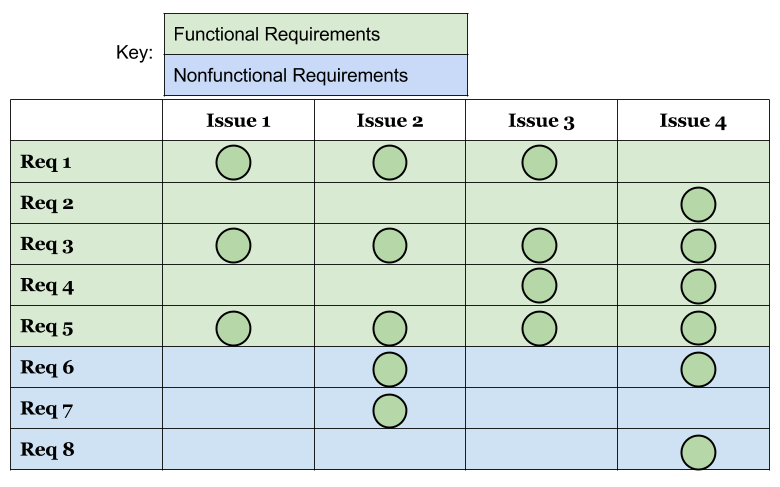
\includegraphics[width=1\textwidth]{images/issues_to_req_matrix.png}
  \caption{Matrix of project requirements to issues project is attempting to
address}
\end{figure}

\chapter{Solution Design: Improved Kepler Visualisation Tool}\label{C:sd}

This section discusses the deliverable visualisation that will be created as part of this project.
The visualisation for this project will be created using Processing, a Java framework for visualisations. As the time is short for this project, extending a previous visualisation that uses the same dataset, the Kepler Visualisation Tool \cite{kepler_github, kepler_article}, will increase the amount of progress that can be made in the time afforded.

The visualisation was designed to emphasis small multiples and filtering of the Exoplanets to display the information more clearly to users. 
\\\\
Instead of the visualisation only answering the 5 key questions as proposed in the proposal, the aim will now be displaying as much of the information in the dataset as possible without detracting from the effectiveness of the visualisation whilst still answering the questions. 
\\\\
This is because the 5 questions did not fully utilize the information in the dataset. 

However I will need to ensure the effectiveness of the visualisation does not become diminished by trying to convey to much information which would lead to cluttering and overlapping in the visualisation, as well as information overload for users. There will also be larger emphasis placed on making the existing system more usable by improving the interaction methods for users. The following list outlines the new requirements for the visualisation being developed. This will be done by 
providing GUI elements for each form of interaction with the system, as well as ensuring all interaction methods are intuitive for users. 
\subsection{Visualisation Layout}

\subsubsection{Component Layout}
As the majority of the interaction and movement of visualisation elements occurs in the center of the window it caused a aspect ratio that was not suitable . It was BETTER to use 2 vertical columns to view and control the visualisation as it had a higher aspect ratio which allowed more of the content to be seen on the screen at once thanks to the fact that the majority of computer screens have a wide ratio.

\begin{figure}[h!]
  \centering
      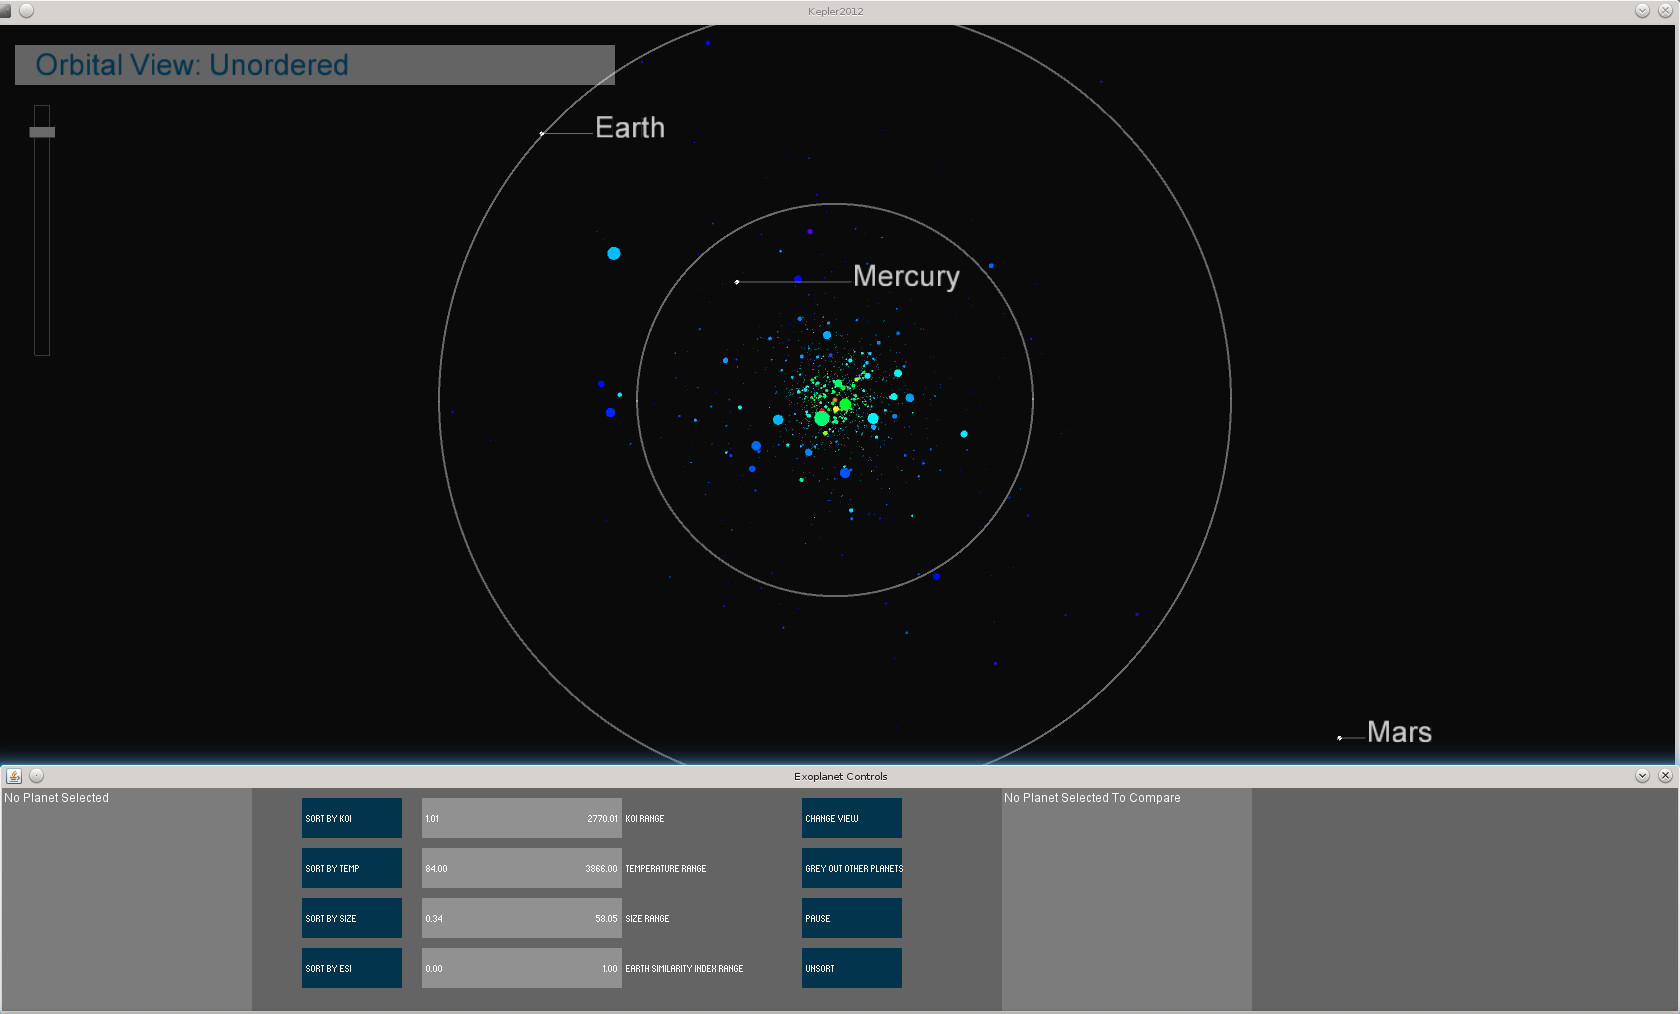
\includegraphics[width=0.8\textwidth]{images/layout_horizontal.jpg}
  \caption{Original Horizontal Layout}  
        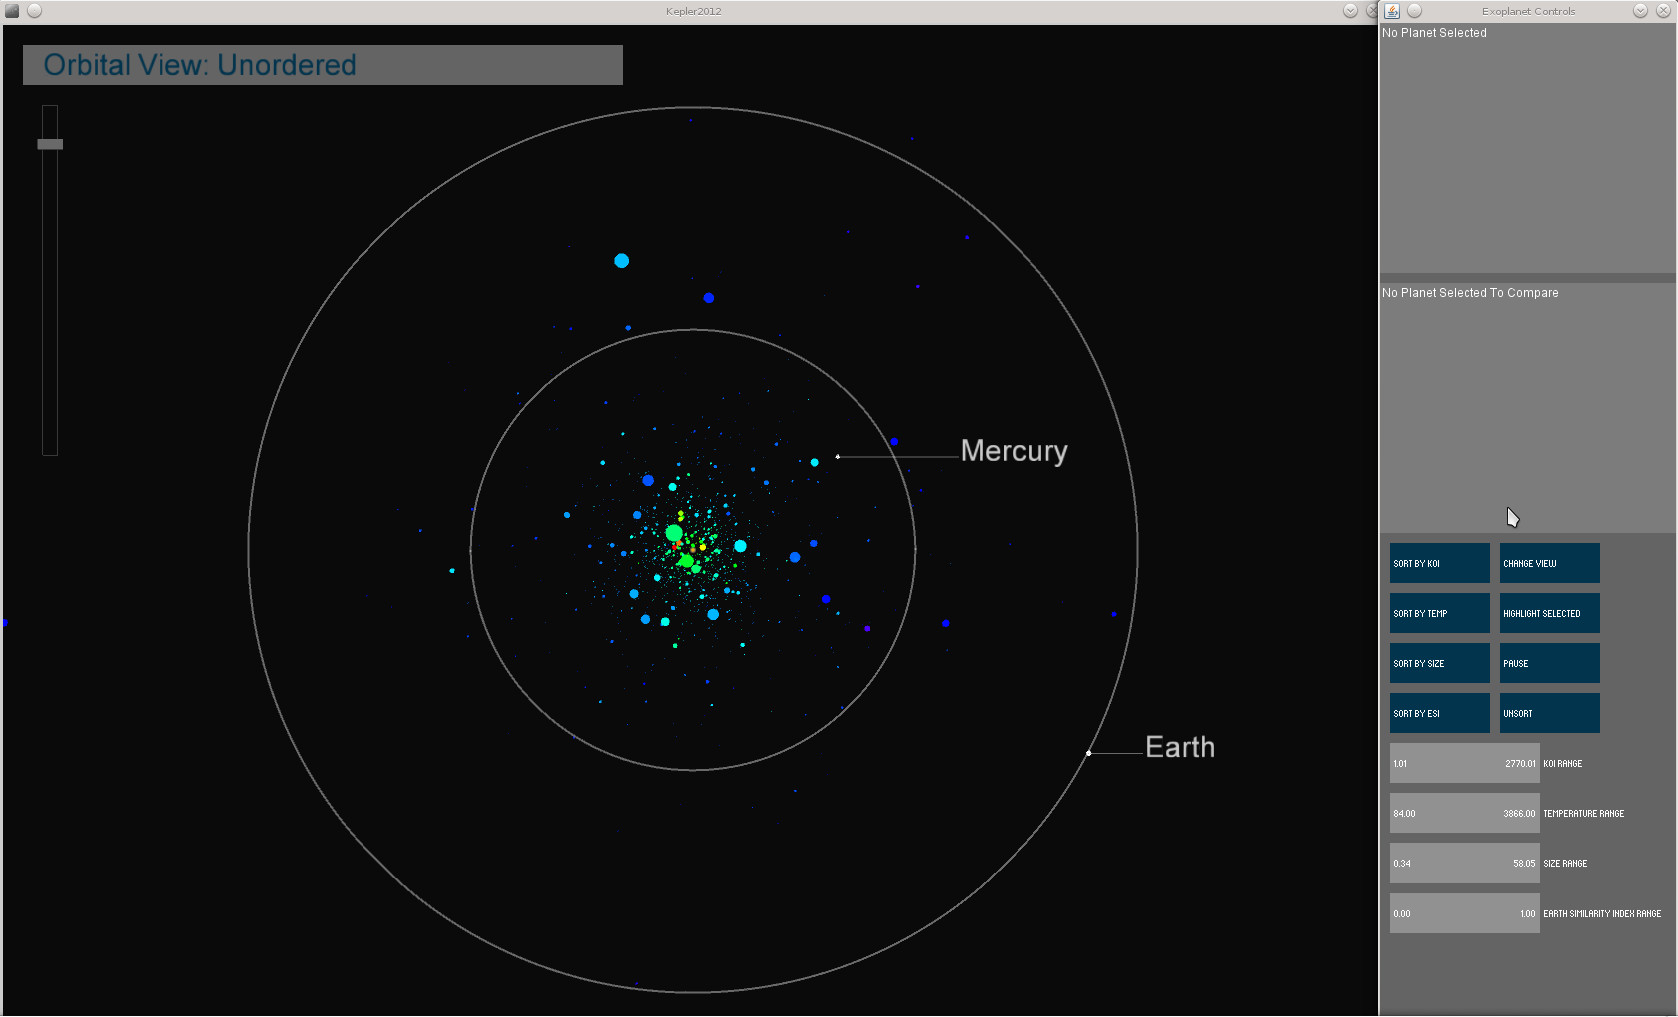
\includegraphics[width=0.8\textwidth]{images/layout_vertical.jpg}
  \caption{Improved Vertical Layout}
\end{figure}

\chapter{Visualisation implementation}\label{C:sd}



\section{Tools and artifacts used}
\subsection{Main system}
In addition to Processing in the main system there was an additional opensource library required for effective user interface components, this library was called
\begin{itemize}
 \item ControlP5 REF~
\end{itemize}


\subsection{Kinect sensor system}
The Microsoft Kinect sensor required 3 additional libraries to integrate with Processing, these were:
\begin{enumerate}
 \item NITE ref~
 \item SimpleOpenNi ref~
\end{enumerate}
These libraries provided drivers to run the Kinect sensor in Processing as well as basic gesture recognition and body tracking. However as the libraries were opensource due to the official Kinect SDK not being compatible with Processing, the gesture recognition was not as user friendy or effective as the official libraries. The effect of this was that the gesture tracking used in the system had to be .... ~
\section{Implementation of planned features}
Image of navigation window

Image of each button

Image of each slider

Image of text boxes

Image of using kinect system

Image of using non kinect system
\section{Extension to initial design}

\section{Problems encountered}
Due to the number of elements that needed to be displayed on screen at any one time (ie 2234 exoplanets), the load placed on a system is very high due to the need to render 2234 eclipses to represent the planets. This uncovered a bug in the processing library in which the memory use of the visualisation would periodically increase until it crashed due to an out of memory exception. After much experimentation of how to overcome this issue, I discovered that rather than trying to render a native elipse shape in processing, if I instead rendered a Scalable Vector Graphic this bug would not manifest. 
\\\\
Libraries used for gesture detection in kinect are opensource in order to work with processing did not have decent detection

Using the Processing framework meant using a non industrial???~ IDE that had many bugs, for example when undoing multiple times in a row the file being modified would periodically become corrupted by lines of code being taken away or inserted into the wrong locations. The solution to this issue was to ensure that I regularily commited any changes to my version controlled system on Github ((REFERBTECE ~)). Doing this meant that if at any time a file became corrupted I could easily see the changes in the file when compared against the precious commit and manually fix the file. 


SCREENSHOT ~
\chapter{Visualisation Evaluation}\label{C:sd}
Following the completion of the implementation stage of this project a final user evaluation was carried out on the visualisation to discover whether the visualisation designed and implemented 



\chapter{Conclusions}\label{C:con}
\section{Future Work}
The work from this project can be taken further in many different ways depending on how it is intended to be used. There is the option of using the system as a terminal that users would use at an observatory or attraction where prior knowledge of the system is limmited and amount of time users would spend on the system would be small. In this case further expanding the user experience and improved Kinect interaction would be benificial as immersion would be the decider on its success. Another option for the system would be for a standalone desktop system that users would use multiple times and so prior knowledge of how to use the system could be expected. This would mean that more complex functionality could be introduced witht he expectation that it could be used by users. The systems current state could me modified to fit into either of these two options.

Occulus rift, look at paper boy


%%%%%%%%%%%%%%%%%%%%%%%%%%%%%%%%%%%%%%%%%%%%%%%%%%%%%%%

\backmatter

%%%%%%%%%%%%%%%%%%%%%%%%%%%%%%%%%%%%%%%%%%%%%%%%%%%%%%%


%\bibliographystyle{ieeetr}
\nocite{*}
\bibliographystyle{acm}
\bibliography{refs}


\end{document}
